\chapter{Υπόβαθρο}

\section{Υπολογιστικό νέφος}
Το υπολογιστικό νέφος (\en{cloud computing}) είναι ένα μοντέλο παροχής
υπολογιστικών πόρων ως υπηρεσίας το οποίο εδραιώνεται πλέον ως κυρίαρχο.
Βασίζεται στην παροχή συγκεντρωμένων, κοινόχρηστων υπολογιστικών πόρων κατ'
απαίτηση (\en{on demand}), μέσω δικτύου. Αυτοί οι φυσικοί πόροι
ανήκουν και διαχειρίζονται από έναν πάροχο υπηρεσιών νέφους (\en{cloud service
provider}) και γίνονται διαθέσιμοι εξ' αποστάσεως σε χρήστες - πελάτες, οι
οποίοι έτσι επιτυγχάνουν χαμηλότερο αρχικό κόστος για υπολογιστική υποδομή,
ευελιξία, κλιμακωσιμότητα, συντομότερο χρόνο \en{deployment} και απλοποιημένη
διαχείριση \cite{wiki:cloud}.

Διακρίνονται τρία βασικά μοντέλα υπηρεσιών \en{cloud} μέσω των οποίων παρέχεται
πρόσβαση στην υποκείμενη υπολογιστική υποδομή, όπως φαίνεται και στο σχήμα
\ref{fig:cloud} \cite{nist-cloud}:
\begin{description}
    \item[\en{Infrastructure-as-a-Service (IaaS)}] όπου γίνονται διαθέσιμοι
        υπολογιστικοί πόροι επεξεργασίας (\en{compute}), αποθήκευσης
        (\en{storage}) και δικτύωσης, όπως εικονικές μηχανές (\en{virtual
        machines}), μονάδες αποθήκευσης, εικονικά δίκτυα και εξισορροπητές
        φόρτου (\en{load balancers}). Αυτό είναι το μοντέλο που προσφέρει το
        μικρότερο επίπεδο αφαίρεσης (\en{abstraction}) παράλληλα με την
        μεγαλύτερη ευελιξία στους χρήστες.
    \item[\en{Platform-as-a-Service (PaaS)}] στο οποίο παρέχεται η δυνατότητα
        στους χρήστες να αναπτύξουν τις εφαρμογές τους λαμβάνοντας ως δεδομένο
        το ``περιβάλλον'' στο οποίο αυτές θα εκτελεστούν. Ουσιαστικά, σε αυτό το
        μοντέλο τους παρέχεται μία υπηρεσία υψηλότερου επιπέδου με την έννοια
        ότι δεν έχουν την ευθύνη της διαχείρισης συστατικών όπως το λειτουργικό
        σύστημα και το σύστημα χρόνου εκτέλεσης (\en{runtime system}), αφήνοντας
        τους να επικεντρωθούν στην εφαρμογή.
    \item[\en{Software-as-a-Service (SaaS)}] όπου πρόκειται για το πιο υψηλό
        επίπεδο αφαίρεσης από την υπολογιστική υποδομή. Σε αυτό δίνεται
        πρόσβαση στους χρήστες σε συγκεκριμένες εφαρμογές, οι οποίες
        διαχειρίζονται πλήρως από τον πάροχο, από την υπολογιστική υποδομή μέχρι
        και την έκδοση και διαμόρφωση της ίδιας της εφαρμογής. Παραδείγματα
        αποτελούν υπηρεσίες ηλεκτρονικής αλληλογραφίας (\en{email}), διαχείρισης
        έργων (\en{project management}) και εφαρμογών γραφείου όπως επεξεργασίας
        εγγράφων και υπολογιστικών φύλλων (\en{spreadsheets}).
\end{description}

\begin{figure}
    \centering
    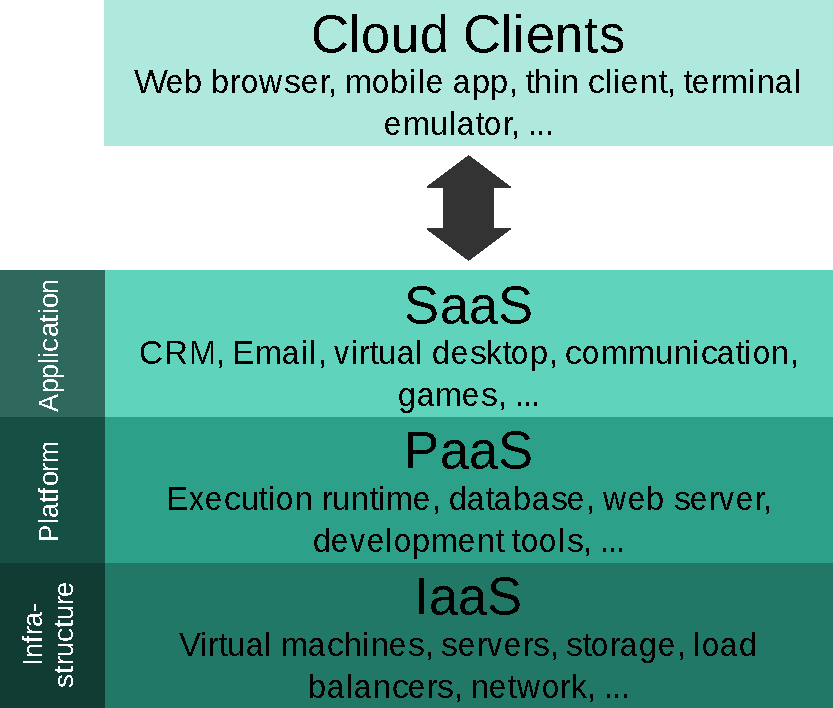
\includegraphics[scale=0.8]{cloud-layers}
    \caption[Μοντέλα παροχής υπηρεσιών \en{cloud}]{Μοντέλα παροχής υπηρεσιών
        \en{cloud}. Πηγή
        \en{\href{https://commons.wikimedia.org/wiki/File:Cloud_computing_layers.svg}{Wikimedia Commons}}.}
    \label{fig:cloud}
\end{figure}

Ένα μοντέλο που έχει κάνει την εμφάνιση του πιο πρόσφατα και έχει ελκύσει
πολλούς χρήστες είναι το λεγόμενο \en{serverless} ή \en{Function-as-a-Service
(FaaS)}. Αυτό ταιριάζει με το \en{PaaS} (θα μπορούσε να θεωρηθεί κομμάτι ή
εξέλιξη του), καθώς όπως υποδηλώνει το όνομα του, αφαιρεί εξ' ολοκλήρου την
ευθύνη του \en{server} από τους χρήστες της υπηρεσίας. Τα τεχνικά χαρακτηριστικά
στα οποία δίνεται έμφαση είναι η αυτόματη κλιμακωσιμότητα από το μηδέν μέχρι και
πολύ μεγάλη κλίμακα καθώς και η άμεση απόκριση σε διακυμάνσεις του φόρτου,
μιας και η εκκίνηση και ο τερματισμός στιγμιοτύπων της εφαρμογής είναι πολύ
γρήγορες διαδικασίες \cite{cloudflare-serverless}. Ένα μειονέκτημα του
\en{serverless} είναι ότι κάποιες μόνο εφαρμογές ταιριάζουν σε αυτό το μοντέλο,
οπότε είναι δυνατό να επωφεληθούν από τα παραπάνω \cite{serverless,
spec-serverless}.

\section{Εικονικοποίηση}
Η τεχνολογία που βρίσκεται κατά κύριο λόγο πίσω από το \en{cloud} είναι αυτή της
εικονικοποίησης (\en{virtualization}). Με αυτήν προστίθεται ένα επίπεδο
αφαίρεσης πάνω από την φυσική υπολογιστική υποδομή, αφού επιτρέπει την
απεικόνιση ενός (συνήθως μεγάλου) φυσικού μηχανήματος (\en{host}) σε
περισσότερα, μικρότερα εικονικά μηχανήματα (\en{virtual machines -- guests}), τα
οποία δημιουργούνται, τροποποιούνται, μεταφέρονται και καταργούνται δυναμικά,
μέσω λογισμικού, θέτοντας τα θεμέλια για τις σύγχρονες υπηρεσίες \en{cloud}
\cite{wiki:hw-virtualization}.

Ως προς τις απαιτήσεις από το λογισμικό που εκτελείται ως \guest{} διακρίνονται
δύο περιπτώσεις:
\begin{description}
    \item[Πλήρης εικονικοποίηση (\en{full virtualization})] όπου ο \guest{} δεν
        αντιλαμβάνεται ότι εκτελείται από ένα εικονικό μηχάνημα. Έτσι, δεν
        απαιτούνται αλλαγές ώστε λογισμικό που έχει δημιουργηθεί για φυσικά
        μηχανήματα να εκτελεστεί σε εικονικά.
    \item[\en{Paravirtualization}] όπου ο \guest{} τροποποιείται ειδικά για την
        εκτέλεση του στο \en{virtual machine}.
\end{description}
Η εικονικοποίηση ήταν παρούσα για δεκαετίες πριν την έλευση του \en{cloud}.
Καθοριστικό σημείο για την υλοποίηση αυτού ήταν η προσθήκη υποστήριξης υλικού
για την εικονικοποίηση στην αρχιτεκτονική \en{x86}, που οδήγησε στην αποδοτική
χρήση της, χωρίς υψηλές απαιτήσεις από το λογισμικό \cite{virtualization-x86}.
Μέχρι εκείνο το σημείο η εικονικοποίηση σε αυτή τη δημοφιλή αρχιτεκτονική
βασιζόταν σε τεχνικές \en{paravirtualization}.

Την ευθύνη για την υλοποίηση της εικονικοποίησης έχει ο λεγόμενος
\en{hypervisor} ή \en{virtual machine monitor (VMM)}. Αυτός είναι συνήθως
λογισμικό, εκτελούμενο στον \host{} με αυξημένα δικαιώματα (\en{privileges}).
Το έργο του περιλαμβάνει την εκκίνηση των εικονικών μηχανών και την
εξομοίωση των ενεργειών που δεν επιτρέπονται σε αυτές, με κυριότερη την
αλληλεπίδραση με τις περιφερειακές συσκευές του συστήματος. Το δεύτερο τυπικά
υλοποιείται με την τεχνική \en{trap and emulate}, όπου συγκεκριμένες εντολές
κατά την εκτέλεση της εικονικής μηχανής προκαλούν \en{traps} στον επεξεργαστή
με συνέπεια τη μεταφορά στον κώδικα του \en{hypervisor}. Εκείνος αναλαμβάνει
να ελέγξει και να εκτελέσει την ενέργεια που επιχείρησε ο \guest{},
επιστρέφοντας κατόπιν τον έλεγχο στο σημείο όπου είχε σταματήσει αυτός. Ο
μηχανισμός ετούτος δίνει στον \en{hypervisor} πλήρη έλεγχο στο μοντέλο
(εικονικών) συσκευών (\en{device model}) του \en{virtual machine}
\cite{wiki:hypervisor}.

Οι \en{hypervisors} διακρίνονται σε δύο πρωταρχικές κατηγορίες (σχήμα
\ref{fig:hypervisors}) \cite{popek74}:
\begin{description}
    \item[Τύπου 1] οι οποίοι εκτελούνται απευθείας πάνω από το φυσικό μηχάνημα,
        αναλαμβάνοντας εξ' ολοκλήρου τη διαχείριση του, πέρα από τη διαχείριση
        των εικονικών μηχανών. Τυπικά αυτοί οι \en{hypervisors} εξαρτώνται από
        έναν \guest{} ειδικού σκοπού, ο οποίος έχει αυξημένα προνόμια σε
        σχέση με τους υπόλοιπους, ώστε να διαχειρίζεται τις συσκευές του
        μηχανήματος, διαθέτοντας τους κατάλληλους οδηγούς (\en{drivers}). Ο πιο
        γνωστός εκπρόσωπος ελεύθερου λογισμικού αυτής της κατηγορίας είναι ο
        \en{Xen} \cite{xen}.
    \item[Τύπου 2] οι οποίοι εκτελούνται ως μέρος ενός τυπικού λειτουργικού
        συστήματος, αναλαμβάνοντας μόνο την εκκίνηση και παρακολούθηση των
        εικονικών μηχανών, ενώ η διαχείριση του \host{} γίνεται από το
        λειτουργικό, ως συνήθως. Σε αυτή την κατηγορία ο κάθε \guest{} συχνά
        είναι απλά μία διεργασία από την σκοπιά του \host{}. Το πιο γνωστό
        παράδειγμα ελεύθερου λογισμικού που ανήκει σε αυτή την κατηγορία είναι
        το \qemu{} \cite{qemu} (τυπικά σε συνδυασμό με το \en{KVM} \cite{kvm},
        το οποίο παρέχει επιτάχυνση υλικού).
\end{description}

\begin{figure}
    \centering
    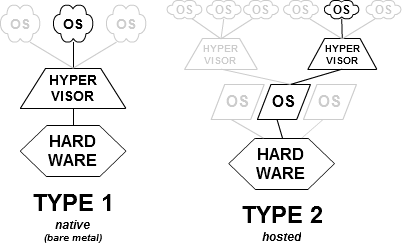
\includegraphics[scale=0.7]{hypervisors}
    \caption[Τύποι \en{hypervisors}]{Τύποι \en{hypervisors}. Πηγή
        \en{\href{https://commons.wikimedia.org/wiki/File:Hyperviseur.png}{Wikimedia Commons}}.}
    \label{fig:hypervisors}
\end{figure}

\section{\en{Unikernels}}
Στην πλέον συνήθη περίπτωση χρήσης της εικονικοποίησης, μπορούμε να θεωρήσουμε
το λογισμικό που υποστηρίζει την εκτέλεση μίας εφαρμογής ως εξής (σχηματικά στο
\ref{fig:components-vm}):
\begin{itemize}
    \item Στον \host{} (\en{kernel space}) εκτελείται ένα γενικού σκοπού
        λειτουργικό σύστημα που έχει απευθείας πρόσβαση στους πόρους του φυσικού
        μηχανήματος και είναι υπεύθυνο γι' αυτούς.
    \item Στον \host{} (τυπικά \en{user space}) εκτελείται επίσης ο
        \en{hypervisor}, αναλαμβάνοντας τη διαχείριση των εικονικών μηχανών που
        αντιστοιχούν στο σύστημα.
    \item Στον \guest{} (\en{kernel space}) εκτελείται και πάλι ένα στιγμιότυπο
        λειτουργικού συστήματος γενικού σκοπού. Αυτό έχει την ευθύνη των πόρων
        του εικονικού μηχανήματος, όπως έχουν ανατεθεί από τον \en{hypervisor}.
    \item Στον \guest{} (\en{user space}) εκτελείται η εφαρμογή, συχνά μαζί με
        συστατικά όπως βιβλιοθήκες τρίτων και συστήματα χρόνου εκτέλεσης
        (\en{runtime systems}).
\end{itemize}
Η στοίβα αυτή λογισμικού περιέχει διπλότυπα και υψηλή πολυπλοκότητα, δύο
στοιχεία τυπικά υπαίτια για προβλήματα όπως η υποβέλτιστη χρησιμοποίηση των
πόρων και οι μειωμένες επιδόσεις λόγω \en{overheads} (πχ \en{mode switches}) στη
συνολική λειτουργία του συστήματος, αλλά και κίνδυνοι ασφαλείας λόγω του
μεγέθους του λογισμικού, από το οποίο μεγάλο μέρος είναι περιττό (πχ οδηγοί του
\en{guest}).
% TODO OPT: any citation?

\begin{figure}
    \begin{subfigure}[b]{0.3\textwidth}
        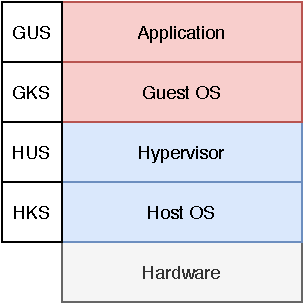
\includegraphics[width=\textwidth]{components-vm}
        \caption{Τυπικό \en{VM}}
        \label{fig:components-vm}
    \end{subfigure}
    \begin{subfigure}[b]{0.3\textwidth}
        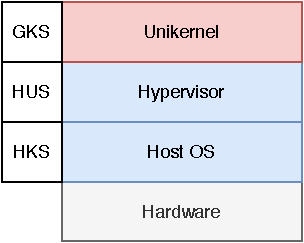
\includegraphics[width=\textwidth]{components-unikernel}
        \caption{\en{Unikernel}}
        \label{fig:components-unikernel}
    \end{subfigure}
    \begin{subfigure}[b]{0.3\textwidth}
        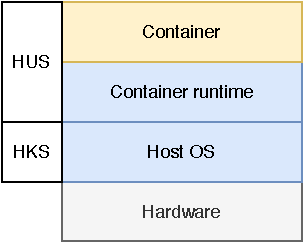
\includegraphics[width=\textwidth]{components-container}
        \caption{\en{Container}}
        \label{fig:components-container}
    \end{subfigure}
    \caption[Σύγκριση μεταξύ αρχιτεκτονικής ``κλασικής'' εικονικής μηχανής,
        \en{unikernel} και \en{container}]{Σύγκριση μεταξύ αρχιτεκτονικής
        ``κλασικής'' εικονικής μηχανής, \en{unikernel} και \en{container}, με
        \en{hypervisor} τύπου 2. Όπου \en{HKS=Host Kernel Space, HUS=Host User
        Space, GKS=Guest Kernel Space} και \en{GUS=Guest User Space}.}
    \label{fig:vm-unikernel-container}
\end{figure}

Μία σύγχρονη προσπάθεια αντιμετώπισης του προηγούμενου προβλήματος είναι τα
\en{unikernels} \cite{mirageos}. Αυτά είναι εκτελέσιμες εικόνες μηχανών
(\en{machine images}) που αποτελούνται από μία εφαρμογή μαζί με όλες τις
απαραίτητες εξαρτήσεις (\en{dependencies}) για την εκτέλεση της, από βιβλιοθήκες
και \en{runtime systems} έως υλοποιήσεις στοίβας δικτύωσης και οδηγούς συσκευών.
Όλα τα παραπάνω βρίσκονται σε έναν κοινό, επίπεδο χώρο διευθύνσεων, χωρίς
διάκριση σε \en{kernel} και \en{user space}, όπως φαίνεται και στο σχήμα
\ref{fig:components-unikernel}. Πρόκειται συνεπώς για ειδικού σκοπού πυρήνες,
κατασκευασμένους ώστε να τρέχουν μία μόνο εφαρμογή, εντός μίας εικονικής
μηχανής, κατόπιν της παρατήρησης ότι συχνά τα \en{virtual machines}
χρησιμοποιούνται για να εξυπηρετήσουν αποκλειστικά μία εφαρμογή.

Τα \en{unikernels} χτίζουν πάνω στην παλαιότερη ιδέα των \en{library operating
systems (OS)}, τα οποία περιγράφονται μαζί με τα πολύ προοδευτικά για την εποχή
τους και επίκαιρα σήμερα \en{exokernels} \cite{exokernel}.
Σε ένα \en{library OS}, η πλειονότητα των λειτουργιών που παραδοσιακά
προσφέρονται ως μέρος ενός μονολιθικού πυρήνα, όπως το σύστημα αρχείων και η
στοίβα δικτύωσης, εξάγονται από αυτόν και γίνονται ανεξάρτητα στοιχεία με την
μορφή βιβλιοθηκών, οι οποίες συνοδεύουν την εφαρμογή. Αυτή η αναδιαμόρφωση
επιτρέπει στην εφαρμογή ελευθερία επιλογής ως προς το ποια από αυτά τα στοιχεία
χρειάζεται να συμπεριλαμβάνει αλλά και ως προς τη συγκεκριμένη υλοποίηση που θα
χρησιμοποιήσει για κάθε ένα από αυτά. Συνεπώς, η εφαρμογή δύναται να
βελτιστοποιήσει τη λειτουργία της μέσω των παραπάνω επιλογών, αλλά ταυτόχρονα
επιβαρύνεται από αυτή την επιπλέον ευθύνη.

Ένα μεγάλο εμπόδιο στην υλοποίηση των \en{unikernels} είναι η ποικιλία συσκευών
και κατά συνέπεια οδηγών που χρειάζονται για την υποστήριξη τους. Αυτό
ξεπερνιέται χάρη στο μοντέλο συσκευών των \en{hypervisors}, το οποίο
περιλαμβάνει λίγες, κοινές και καλώς καθορισμένες συσκευές. Ένα άλλο εμπόδιο
είναι η πολυπλοκότητα της διαδικασίας ταιριάσματος των διαφορετικών στοιχείων
(\en{components}) μεταξύ τους και της κατασκευής της τελικής εκτελέσιμης εικόνας
από αυτά. Για την αντιμετώπιση του διατίθεται πληθώρα λύσεων, με κάθε μία
να σχηματίζει ένα λεγόμενο \en{unikernel framework}. Πρακτικά όλα αυτά είναι
έργα ελεύθερου λογισμικού, με καθένα να προσφέρει συνήθως ένα σύνολο
βιβλιοθηκών για χρήση από τις εφαρμογές των χρηστών, όπως επίσης και τα
απαραίτητα εργαλεία για το χτίσιμο των εικόνων. Κάθε ένα από αυτά τα
\en{frameworks} ακολουθεί τυπικά μία από δύο βασικές προσεγγίσεις:
\begin{itemize}
    \item Αγνή (\en{clean-slate}), που χαρακτηρίζεται από την παροχή
        μη-πρότυπων (\en{custom}) διεπαφών εφαρμογής (\en{APIs}). Επίσης, σε
        αυτή την περίπτωση ο κώδικας των βιβλιοθηκών αλλά και της εφαρμογής
        είναι γραμμένος στην ίδια γλώσσα. Σαφές μειονέκτημα αποτελεί το γεγονός
        ότι οι εφαρμογές πρέπει να γραφτούν από την αρχή στη γλώσσα και με χρήση
        του \en{API} του εκάστοτε \en{framework}.
    \item Συμβατή (\en{compatible}), που χαρακτηρίζεται από την παροχή
        παραδοσιακών διεπαφών (πχ \en{POSIX}), επιτρέποντας σε ήδη υπάρχουσες
        εφαρμογές να εκτελεστούν με ελάχιστες έως καθόλου τροποποιήσεις,
        ανεξάρτητα από τη γλώσσα στην οποία έχουν αρχικά γραφτεί (\en{binary
        compatibility}). Εν προκειμένω, το μεγαλύτερο μειονέκτημα είναι η
        δέσμευση με συχνά παλαιωμένες διεπαφές, που δεν επιτρέπουν την πλήρη
        εκμετάλλευση του δυναμικού των \en{unikernels}.
\end{itemize}
Ενδεικτικά, στην πρώτη κατηγορία ανήκουν το \en{MirageOS} \cite{mirageos} και το
\en{IncludeOS} \cite{includeos}, ενώ στη δεύτερη βρίσκει κανείς τα \en{RumpRun}
\cite{rumprun}, \osv{} \cite{osv} και \en{HermiTux} \cite{hermitux}. Συνολικά
υπάρχει ένας αρκετά μεγάλος αριθμός \en{unikernel frameworks}. Η δημοτικότητα
τους κυμαίνεται, χωρίς κάποιο να επικρατεί, ενώ ποικίλουν τα στάδια συντήρησης
τους (από ενεργά έως πρακτικά εγκαταλελειμμένα) όπως και οι καταβολές τους
(ακαδημαϊκά, εταιρικά ή και προσωπικά έργα).

% TODO OPT: Mention edge use case for unikernels? (not here necessarily)

\subsection{\osv{}}
Το \osv{} είναι ένα \en{unikernel framework} που υποστηρίζει εφαρμογές γραμμένες
για το \linux{}, ενώ παρέχει και δικό του \en{API}, το οποίο μπορούν
προαιρετικά να χρησιμοποιήσουν νέες εφαρμογές \cite{osv}. Εξ' αρχής σχεδιάστηκε
με το \en{cloud} κατά νου, προκειμένου να χρησιμοποιηθεί ιδίως από σύγχρονες
εφαρμογές που συχνά συναντώνται σε αυτό. Ως έργο ξεκίνησε από την \en{Cloudius
Systems} (μετέπειτα \en{ScyllaDB}), αλλά τα τελευταία χρόνια συντηρείται εξ'
ολοκλήρου από μία μικρή ομάδα εθελοντών, ενώ είναι διαθέσιμο με τους όρους της
άδειας \en{BSD}. Η κοινότητα του χρησιμοποιεί μία \en{mailing list}%
\footnote{\en{\url{https://groups.google.com/forum/\#!forum/osv-dev}}}
για την ανάπτυξη του: υποβολή \en{patches}, \en{code review} και γενική
συζήτηση.

Αν και τα κομμάτια που παρέχει το ίδιο είναι γραμμένα σε \en{C++}, ενώ
χρησιμοποιεί κομμάτια από άλλα έργα που ως επί το πλείστον έχουν γραφτεί σε
\en{C}, δεν θέτει περιορισμούς στις εφαρμογές που υποστηρίζει. Το
τελευταίο βέβαια ισχύει αρκεί αυτές να μην κάνουν χρήση λειτουργιών που από τη
φύση τους δεν υλοποιούνται στα \en{unikernels}: κλήσεις συστήματος στην
οικογένεια των \texttt{\en{fork()}} και \texttt{\en{exec()}}. Επίσης, διαθέτει
υποστήριξη για πολλούς \en{hypervisors}, μεταξύ των οποίων οι \qemu{}/\en{KVM},
\en{Xen} και \en{firecracker} \cite{firecracker}.
Ως γενική παρατήρηση, είναι από τα πλέον εξελιγμένα \en{unikernels} από πλευράς
λειτουργιών, και πιο ``βαρύ'' (\en{heavy-weight}) κατά συνέπεια.

Συγκεκριμένα όσον αφορά τα συστήματα αρχείων, το \osv{} προσφέρει πολλές
επιλογές. Κατ' αρχάς, διαθέτει ένα ολοκληρωμένο εικονικό σύστημα αρχείων
(\en{VFS, Virtual File System}), το οποίο έχει βασίσει σε αυτό του \en{Prex}
\cite{prex}.
Κάτω από αυτό βρίσκονται οι υλοποιήσεις των διάφορων συστημάτων αρχείων που
διαθέτει, τα οποία διακρινόμενα σε δύο κατηγορίες είναι:
\begin{itemize}
    \item Τα \en{pseudo-file systems}, αντίστοιχα με αυτά στο \linux{}:
        \en{devfs, procfs, sysfs} και \en{ramfs}.
    \item Τα συμβατικά συστήματα αρχείων: \en{ZFS} (βασισμένο σε υλοποίηση του
        \en{FreeBSD}), \en{rofs} (\en{custom, read-only file system} με απλή
        λογική \en{caching}) και \en{NFS} (χρησιμοποιώντας τη \en{libnfs})
        \cite{libnfs}.
\end{itemize}

% TODO OPT: More technical: virtual memory, virtual file system, network stack,
% aarch64, musl.

\subsection{Εναλλακτικές}
Όπως είναι αναμενόμενο, έχουν προταθεί και εναλλακτικές προσεγγίσεις στο
πρόβλημα του \en{bloated virtualized software stack}. Με διαφορά η πιο
διαδεδομένη αυτήν την περίοδο είναι εκείνη των \en{containers}. Αυτά ανήκουν
στην ευρεία κατηγορία της εικονικοποίησης σε επίπεδο λειτουργικού συστήματος
(\en{OS-level virtualization} \cite{wiki:os-level-virtualization}, σχηματικά στο
\ref{fig:components-container}).

Υπάρχουν πολλές τεχνικές υλοποίησης των \en{containers}, οι περισσότερες εκ των
οποίων βασίζονται σε μηχανισμούς του \linux{} \en{kernel} όπως τα \en{cgroups}
και \en{namespaces} προκειμένου να παρέχουν απομόνωση μεταξύ των διαφορετικών
\en{containers}. Το κοινό όλων τους είναι ότι οι εφαρμογές που τρέχουν σε όλα
τα \en{containers} του ίδιου μηχανήματος μοιράζονται το ίδιο στιγμιότυπο πυρήνα
(\en{kernel}). Θα μπορούσαμε να πούμε ότι σε αυτή την περίπτωση έχουμε ένα
\en{kernel}, αλλά πολλαπλά \en{user spaces}.

Στα σημαντικά πλεονεκτήματα των \en{containers} είναι ότι είναι πολύ πιο
``ελαφριά'' από τις εικονικές μηχανές: πολύ χαμηλότερος χρόνος εκκίνησης (από
ένα \en{virtual machine} με \guest{} γενικού σκοπού), σε συνδυασμό με μεγαλύτερη
ευελιξία και πιο αποδοτική χρήση των πόρων, με αποτέλεσμα να μπορούν να
επιτύχουν υψηλότερη πυκνότητα (στιγμιότυπα που εκτελούνται ταυτόχρονα στο ίδιο
φυσικό μηχάνημα). Το σημαντικότερο μειονέκτημα τους είναι ότι προσφέρουν κατ'
αρχήν πολύ πιο ασθενή απομόνωση από ότι οι εικονικές μηχανές, λόγω του κοινού
πυρήνα που τα εξυπηρετεί απευθείας \cite{lightvm}.

% TODO OPT: Αll other approaches (lw virt, user-space kernels).

% TODO OPT: Compare native, legacy virtual, unikernel and container execution in
% terms of flexibility, security (separation) and efficiency / scalability.

\section{Κοινόχρηστα συστήματα αρχείων}
Τα ``κλασικά'' συστήματα αρχείων είναι υλοποιημένα πάνω από συσκευές \en{block}
(``δίσκους''), συνδεδεμένες μέσω ενός διαύλου (\en{bus}) τοπικού συστήματος.
Το λογισμικό που τα υλοποιεί είναι συνήθως μέρος του πυρήνα ενός λειτουργικού
συστήματος, το οποίο θεωρεί ότι έχει την αποκλειστικότητα επί του συστήματος
αρχείων από τη στιγμή της προσάρτησης (\en{mount}) μέχρι και την στιγμή της
αποπροσάρτησης (\en{unmount}) αυτού. Το τελευταίο αποτελεί σε πολλές περιπτώσεις
έναν περιορισμό, ο οποίος ήδη από την έλευση της δικτύωσης των υπολογιστών
επιδιώχθηκε να αρθεί, επιτρέποντας την ταυτόχρονη χρήση ενός συστήματος αρχείων
από περισσότερους υπολογιστές, καθιστώντας το κοινό. Ο πιο γνωστός και μεταξύ
των παλαιότερων εκπροσώπων κοινόχρηστων συστημάτων αρχείων είναι το \en{NFS
(Network File System)} \cite{nfs},
ενώ η κατηγορία έχει εμπλουτιστεί σημαντικά με την επέκταση των κατανεμημένων
υπολογιστικών συστημάτων τις τελευταίες δεκαετίες.

Με την εικονικοποίηση έχουμε μία ιδιαίτερη περίπτωση πολλαπλών, συνδεδεμένων
μηχανημάτων: του \host{} και των \en{virtual machines} που εκτελούνται σε αυτόν.
Το ζητούμενο του κοινόχρηστου συστήματος αρχείων μεταξύ τους είναι συνεπώς κι
εδώ παρόν και μάλιστα, λόγω της συνύπαρξης στο ίδιο φυσικό μηχάνημα είναι μία
πολύ συχνή απαίτηση. Εξάλλου, το σύστημα αρχείων στον \host{} αποτελεί έναν
ακόμα πόρο του, οπότε είναι αναμενόμενο να μπορεί να δοθεί πρόσβαση σε αυτόν από
τους \en{guests}.

Οι περισσότερες λύσεις για κοινόχρηστα συστήματα αρχείων μεταξύ \host{} και
\guest{} βασίζονται στα ήδη υπάρχοντα, δικτυακά συστήματα αρχείων, μη
διακρίνοντας αυτή την περίπτωση από εκείνη των χωριστών \en{hosts}. Αυτή η
προσέγγιση λειτουργεί βεβαίως βασιζόμενη στη σύνδεση δικτύου μεταξύ των μερών,
πλήρως επαναχρησιμοποιώντας ήδη υπάρχουσες λύσεις. Ένα δημοφιλές παράδειγμα
κοινόχρηστου συστήματος αρχείων στο πλαίσιο της εικονικοποίησης είναι το
\en{VirtFS} \cite{virtfs}, που εκμεταλλεύεται το πρωτόκολλο \en{9P} \cite{9p}.
Αν και το τελευταίο είναι ένα δικτυακό πρωτόκολλο, στην πράξη το \en{VirtFS}
δεν χρησιμοποιεί το δίκτυο στο επίπεδο μεταφοράς του, κάτι που του επιτρέπει
βελτιωμένες επιδόσεις.

Αξίζει να αναφέρουμε ότι και στην περίπτωση των \en{containers} είναι ιδιαίτερα
συχνή η απαίτηση της πρόσβασης σε κοινό σύστημα αρχείων με τον \host{}. Ένας
τρόπος με τον οποίο αυτό επιτυγχάνεται στο \en{Docker} \cite{docker}
(με διαφορά το πιο δημοφιλές \en{container runtime}) είναι η χρήση των λεγόμενων
\en{bind mounts} \cite{docker:bind-mounts},
που εκμεταλλεύονται τον κοινό πυρήνα για να προσαρτήσουν έναν κατάλογο του
\host{} εντός του συστήματος αρχείων του \en{container}.

\section{\viofs{}}
Η κοινή υποκείμενη μνήμη ανάμεσα στον \host{} και τους \en{guests} είναι ένα
στοιχείο το οποίο δεν εκμεταλλεύονται πλήρως τα υπάρχοντα κοινόχρηστα συστήματα
αρχείων. Αυτό έρχεται να αλλάξει το \viofs{} \cite{virtiofs-website}, το οποίο
έχει σχεδιαστεί εξ' αρχής με ετούτο το σκοπό. Το στοιχείο που το διαφοροποιεί
από τα υπόλοιπα είναι ότι δεν εξαρτάται από το δίκτυο στο επίπεδο μεταφοράς,
όπου χρησιμοποιεί το \en{virtio}, ούτε όμως και στο επίπεδο του πρωτοκόλλου,
όπου βασίζεται στο \en{FUSE}. Αυτές οι δύο επιλογές του επιτρέπουν καλύτερες
επιδόσεις, αλλά και σημασιολογία (\en{semantics}) τοπικού συστήματος αρχείων,
μια διαφορά που εκδηλώνεται για παράδειγμα σε θέματα συνοχής (\en{coherence}).

Η υπάρχουσα υλοποίηση του \viofs{} στο \qemu{} έχει μία αρχιτεκτονική
ιδιαιτερότητα. Ενώ τυπικά η υλοποίηση των συσκευών περιέχεται εξ' ολοκλήρου στο
\qemu{}, εδώ ένα σημαντικό μέρος της υλοποίησης είναι διαχωρισμένο, υλοποιημένο
στο λεγόμενο \en{virtiofsd (virtio-fs daemon)}, μία ανεξάρτητη διεργασία που
αναλαμβάνει όλες τις λειτουργίες του συστήματος αρχείων στον \host{}, ενώ το
\qemu{} έχει μόνο την ευθύνη της εικονικής συσκευής. Αυτή η αρχιτεκτονική
έχει αφενός το όφελος υψηλότερης ασφάλειας, καθώς ο \en{virtiofsd} μπορεί
περιοριστεί σε ένα \en{sandbox} χρησιμοποιώντας μηχανισμούς του \host{}
(\en{namespaces, seccomp}). Αφετέρου, είναι αρθρωτή (\en{modular}), επιτρέποντας
εύκολη εναλλαγή ανάμεσα σε διαφορετικές υλοποιήσεις του \en{virtiofsd} (πχ με
μία που αντί πρόσβασης στο σύστημα αρχείων του \host{} να χρησιμοποιεί κάποιο
κατανεμημένο σύστημα αρχείων). Ο διαχωρισμός της υλοποίησης σε περισσότερες
διεργασίες καθίσταται δυνατός χάρη στο \en{vhost-user} πρωτόκολλο
\cite{vhost-user},
το οποίο με τη σειρά του εξελίσσει την ιδέα του \en{vhost} στο \qemu{}
\cite{stefanha:vhost}. Η ώθηση των συσκευών εκτός του \en{VMM} έχει αρκετά
πλεονεκτήματα και είναι μία τάση που αναμένεται να ακολουθηθεί και στο μέλλον
\cite{stefanha:out-of-process-dev}.

\subsection{\en{Virtio}}
Το \en{virtio} είναι μία πρότυπη (\en{standard}) προδιαγραφή συσκευών,
αποκλειστικά για \en{virtualized} περιβάλλοντα \cite{virtio}. Χαίρει ευρείας
υποστήριξης και είναι η πλέον αποδεκτή λύση στο πρόβλημα του κατακερματισμού
(\en{fragmentation}) των μοντέλων συσκευών σε αυτά. Προσφέρει έναν αποδοτικό και
επεκτάσιμο μηχανισμό, ενώ βασίζεται σε ορολογία και μηχανισμούς φυσικών
συσκευών, διευκολύνοντας την υποστήριξη και επιτρέποντας την επαναχρησιμοποίηση
από υπάρχουσες υλοποιήσεις οδηγών στους \en{guests}.

Το πρότυπο έχει δύο βασικούς άξονες:
\begin{description}
    \item[Το επίπεδο μεταφοράς] το οποίο ορίζει έναν γενικό τρόπο για την
        ανακάλυψη (\en{discovery}), διαμόρφωση (\en{configuration}) και κανονική
        λειτουργία (αμφίδρομη μεταφορά δεδομένων) των συσκευών. Η τελευταία
        γίνεται μέσω των λεγόμενων \en{virtqueues}, βασιζόμενη στην κοινή μνήμη
        μεταξύ \guest{} και \en{hypervisor}. Το επίπεδο μεταφοράς, το οποίο
        κατ' αρχήν ορίζεται αφηρημένα, εξειδικεύεται με τρεις υλοποιήσεις:
        δίαυλο \en{(bus) PCI}, \en{memory-mapped I/O (MMIO)} και \en{channel
        I/O} (για περιπτώσεις βασισμένες στην αρχιτεκτονική \en{S/390} της
        \en{IBM}).
    \item[Το σύνολο των συσκευών] που χτίζεται πάνω από το επίπεδο μεταφοράς,
        καθορίζοντας για κάθε συσκευή τα διαθέσιμα πεδία διαμόρφωσης
        (\en{configuration fields}) της, το πλήθος των \en{virtqueues} που
        χρησιμοποιεί και τα μηνύματα που μεταφέρονται μέσω αυτών για τη
        λειτουργία της.
\end{description}

\subsection{\en{FUSE}}
Το \en{FUSE (Filesystem in Userspace)} είναι ένα πρωτόκολλο που συστήθηκε στο
\linux{} προκειμένου να επιτρέψει την υλοποίηση συστημάτων αρχείων στο
\en{user space} αντί εντός του πυρήνα \cite{fuse}.
Όπως φαίνεται και στο σχήμα \ref{fig:fuse}, στην αρχιτεκτονική του η υλοποίηση
των λειτουργιών του συστήματος αρχείων γίνεται από ένα \en{user space daemon}
που επικοινωνεί σύμφωνα με το πρωτόκολλο με τον πυρήνα μέσω μίας ειδικής
συσκευής χαρακτήρων (\texttt{\en{/dev/fuse}}). Όταν το \en{kernel} δέχεται
\en{VFS} αιτήματα που αντιστοιχούν σε κάποιο \en{FUSE} σύστημα αρχείων, τα
προωθεί στο κατάλληλο \en{daemon}, που έχει το ρόλο του \en{backend}.

\begin{figure}
    \centering
    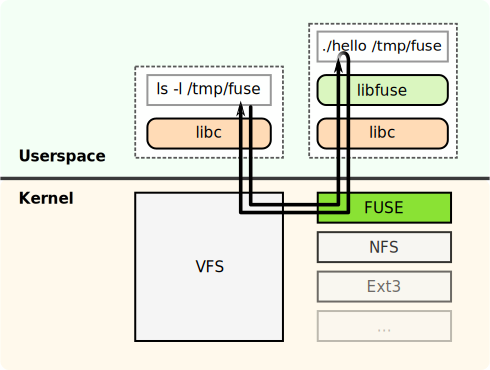
\includegraphics[width=\textwidth]{fuse}
    \caption[Δομή του \en{FUSE} στο \linux{}]{Δομή του \en{FUSE} στο
        \linux{}. Από τον \en{Sven}
        (\en{\url{https://commons.wikimedia.org/wiki/User:Sven}}) υπό την άδεια
        \en{CC-BY-SA 3.0}
        (\en{\url{https://creativecommons.org/licenses/by-sa/3.0/legalcode}}).
        Πηγή
        \en{\url{https://commons.wikimedia.org/wiki/File:FUSE_structure.svg}}.}
    \label{fig:fuse}
\end{figure}

Στο πλαίσιο του \viofs{}, το \en{FUSE} αξιοποιείται ως πρωτόκολλο επικοινωνίας
των αιτημάτων συστήματος αρχείων με τη συσκευή. Έτσι, κατά κάποιον τρόπο η
αρχιτεκτονική του μοιάζει με την κλασική αρχιτεκτονική του \en{FUSE} με τη
διαφορά ότι πελάτης (\en{client}) είναι ο \en{guest} αντί του πυρήνα, ενώ η
επικοινωνία γίνεται μέσω \en{virtio} αντί της \en{FUSE} συσκευής χαρακτήρων.
Στην πράξη όμως, το \viofs{} και το τυπικό \en{FUSE} είναι ασύμβατα μεταξύ τους,
με το \viofs{} να περιλαμβάνει τροποποιήσεις και επεκτάσεις στο πρωτόκολλο του
\en{FUSE}. Επίσης, το μοντέλο ασφαλείας (\en{security model}) είναι διαφορετικό
(ουσιαστικά ανεστραμμένο), μιας και στο \viofs{} ο \en{client} (\guest{}) είναι
αναξιόπιστος, ενώ στο \en{FUSE} συμβαίνει το αντίθετο (υπάρχει εξ' ορισμού
εμπιστοσύνη στον πυρήνα πάνω στον οποίο τρέχει ο \en{daemon}). Το τελευταίο
μεταφράζεται σε πιο ασφαλή χειρισμό των αιτημάτων σε ένα \viofs{} \en{device
backend} από ότι σε ένα \en{FUSE backend}.

% TODO OPT: Protocol description

\subsection{\en{DAX window}}
Ο τρόπος που διαθέτει το \en{FUSE} για την ανάγνωση και εγγραφή αρχείων είναι
μέσω των \en{FUSE\_READ} και \en{FUSE\_WRITE requests} αντίστοιχα. Αυτά
προβλέπουν την αντιγραφή των δεδομένων και, στην περίπτωση του \viofs{}
συνεπάγονται και εξόδους της εικονικής μηχανής (\en{VM exits}). Καθώς όμως αυτές
οι δύο λειτουργίες είναι κεντρικές στο \en{data path}, η βελτιστοποίηση τους
είναι απαραίτητη. Προς αυτή την κατεύθυνση το \viofs{} συστήνει το λεγόμενο
\en{DAX window}: ένα ``παράθυρο'' κοινής μνήμης ανάμεσα στον \host{} και το
\guest{}, στο οποίο απεικονίζονται τα περιεχόμενα των αρχείων, δίνοντας στον
\guest{} απευθείας πρόσβαση σε αυτά. Με αυτόν τον τρόπο επιτυγχάνεται αποφυγή
των αντιγραφών (και παράκαμψη της \en{page cache} του \en{guest} στην περίπτωση
του \linux{}), ενώ πλέον δεν συνεπάγεται κάθε λειτουργία ανάγνωσης ή εγγραφής
έξοδο από την εκτέλεση της εικονικής μηχανής.

\begin{figure}
    \centering
    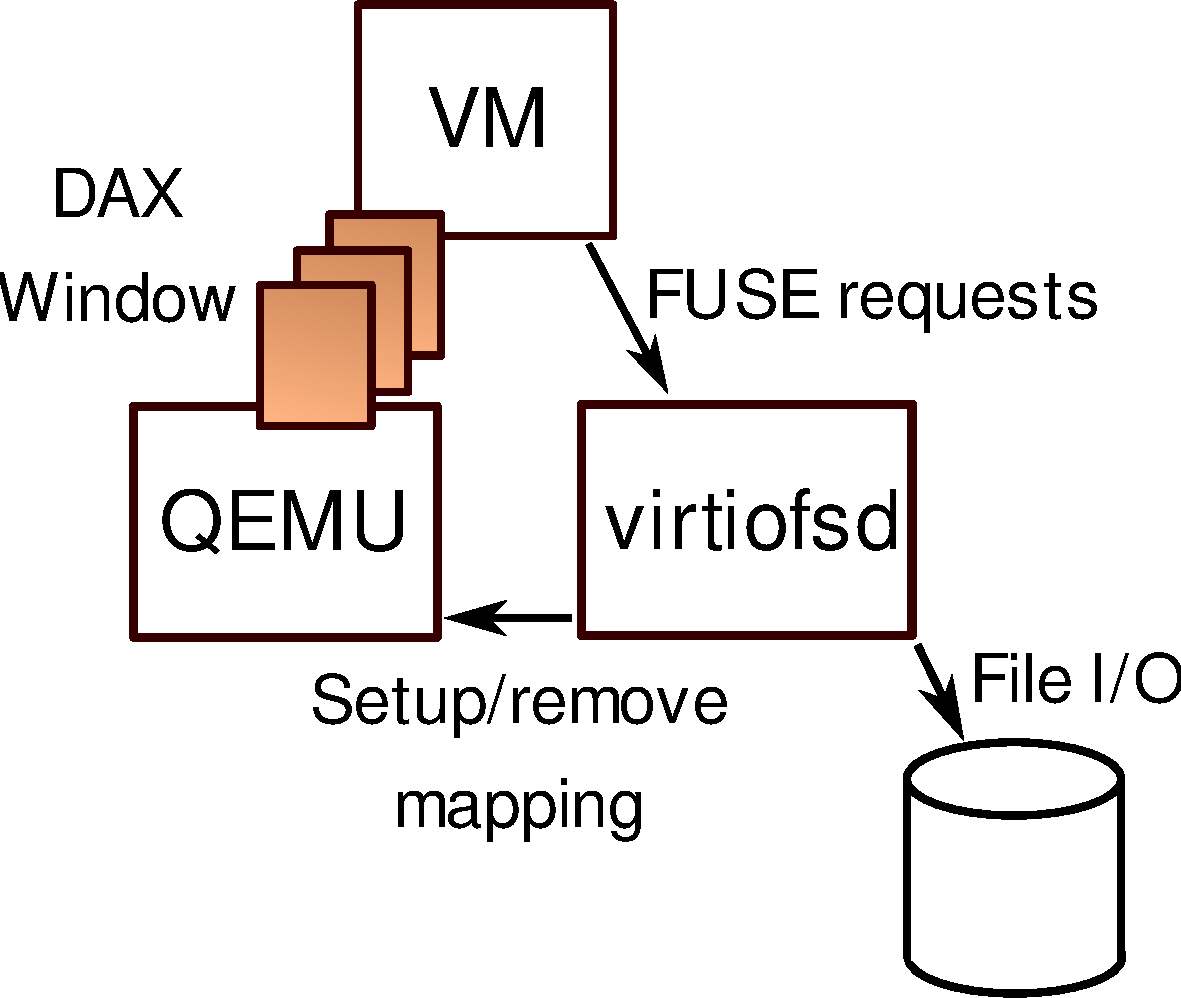
\includegraphics[scale=0.5]{dax-architecture}
    \caption[Αρχιτεκτονική του \en{DAX window} στο \viofs{}]{Αρχιτεκτονική του
        \en{DAX window} στο \viofs{}. Από τον \en{Stefan Hajnoczi}
        (\en{\url{https://vmsplice.net/}}) υπό την άδεια \en{CC-BY-SA 4.0}
        (\en{\url{https://creativecommons.org/licenses/by-sa/4.0/legalcode}}).
        Πηγή
        \en{\url{https://gitlab.com/virtio-fs/virtio-fs.gitlab.io/-/blob/master/architecture.svg}}.}
    \label{fig:dax-architecture}
\end{figure}

% TODO OPT: DAX subsystem in Linux, pmem

Για την υλοποίηση της λειτουργικότητας του \en{DAX window} κατ' αρχάς
επεκτείνεται το \en{FUSE} πρωτόκολλο με μηνύματα για την εγκαθίδρυση και την
κατάργηση απεικονίσεων (\en{mappings}). Αυτά τα μηνύματα χρησιμοποιεί ο \guest{}
προκειμένου ο \en{virtiofsd} (κατόπιν των απαραίτητων ελέγχων) να καθοδηγήσει το
\qemu{} μέσω της μεταξύ τους σύνδεσης να πραγματοποιήσει καθεαυτή τη λειτουργία
(δημιουργία ή κατάργηση απεικόνισης). Σχηματικά τα παραπάνω φαίνονται
στο \ref{fig:dax-architecture}.
